%================================================================
\section{Appendix}\label{sec:Appendix A}
%================================================================

%----------------------------------------------------------------
\subsection{Additional Results}\label{app:additional_results}
%---------------------------------------------------------------- 

\autoref{fig:alpha_epoch_rwm}

\begin{figure}[!htb]
\centering
\subfloat[]{{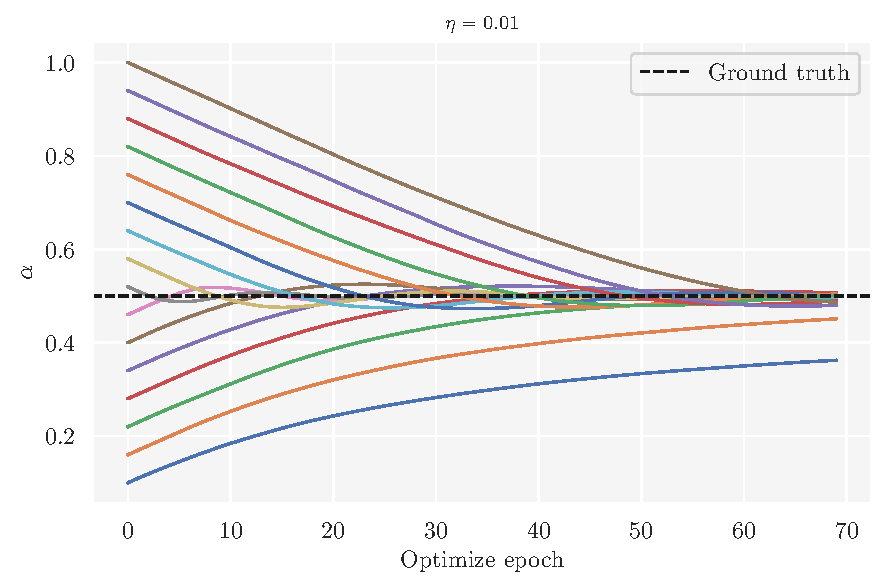
\includegraphics[scale=0.5]{latex/figures/alpha_epoch_rwm_ashonib_eta001.pdf}}}
\qquad
\subfloat[]{{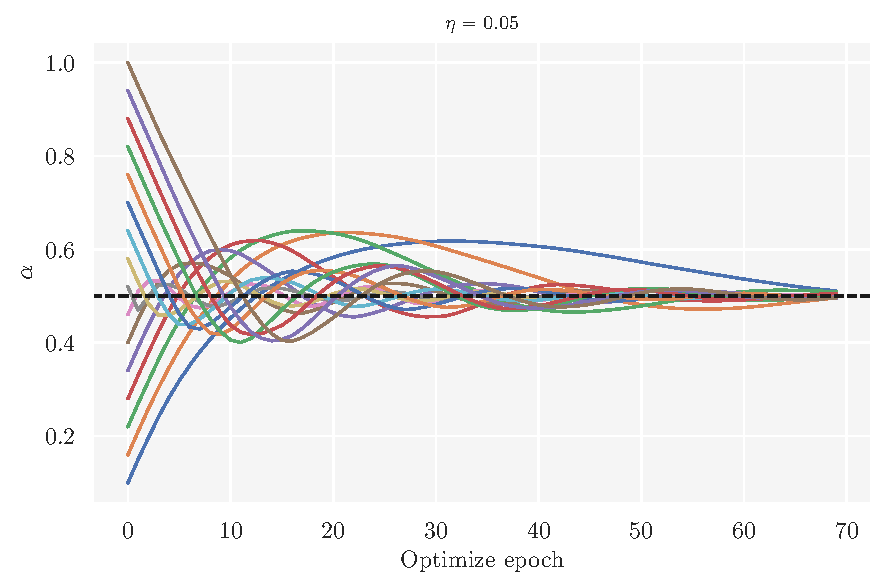
\includegraphics[scale=0.5]{latex/figures/alpha_epoch_rwm_ashonib_eta005.pdf}}}
\qquad
\subfloat[]{{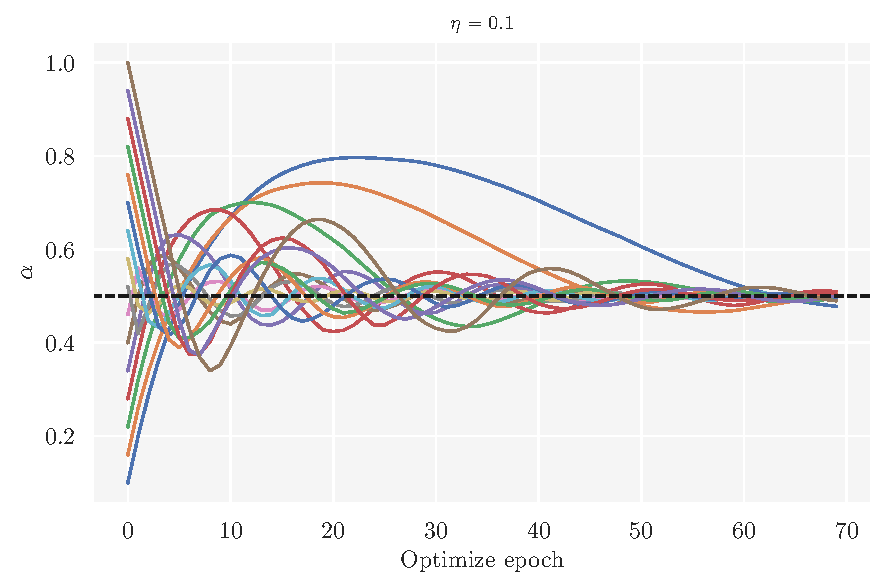
\includegraphics[scale=0.5]{latex/figures/alpha_epoch_rwm_ashonib_eta01.pdf}}}
\qquad
\subfloat[]{{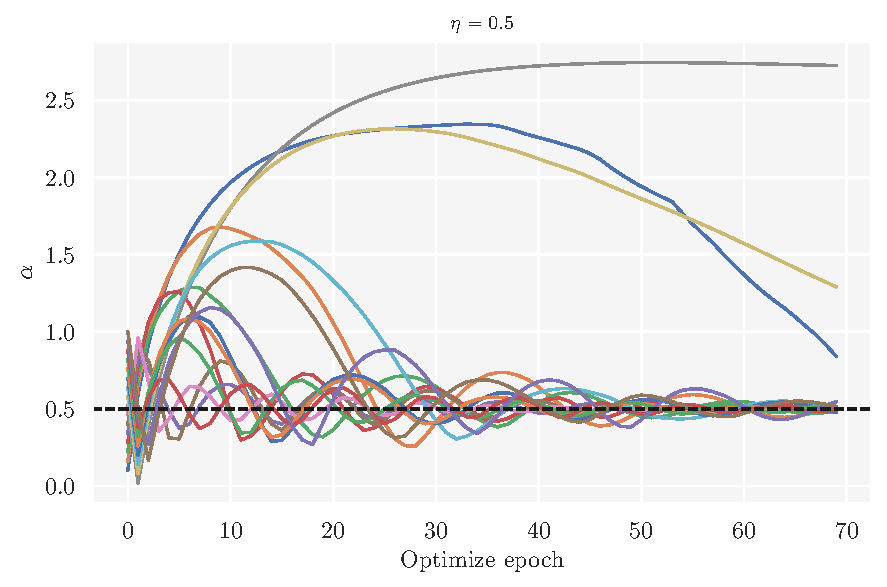
\includegraphics[scale=0.5]{latex/figures/alpha_epoch_rwm_ashonib_eta05.pdf}}}
\caption{figure text}
\label{fig:alpha_epoch_rwm}
\end{figure}

\autoref{fig:alpha_epoch_lmh}

\begin{figure}[!htb]
\centering
\subfloat[]{{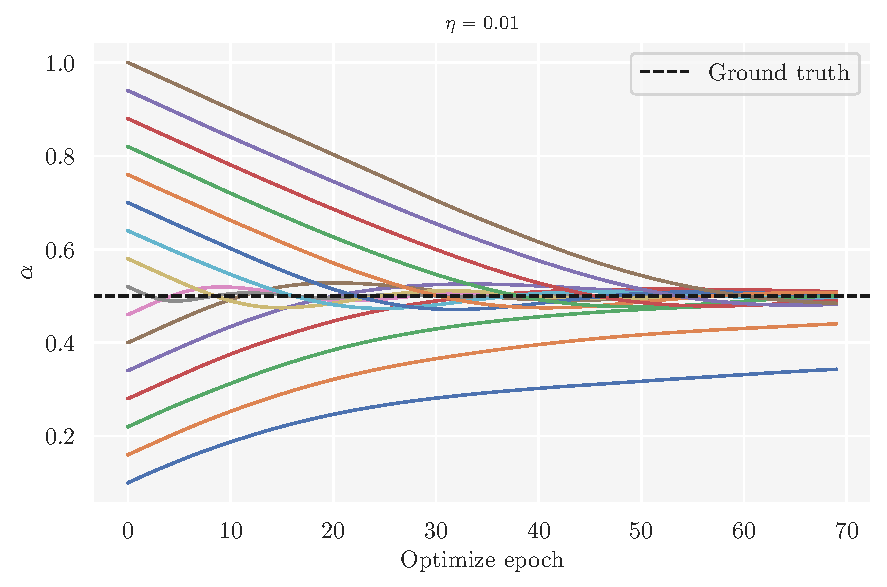
\includegraphics[scale=0.5]{latex/figures/alpha_epoch_lmh_ashonib_eta001.pdf}}}
\qquad
\subfloat[]{{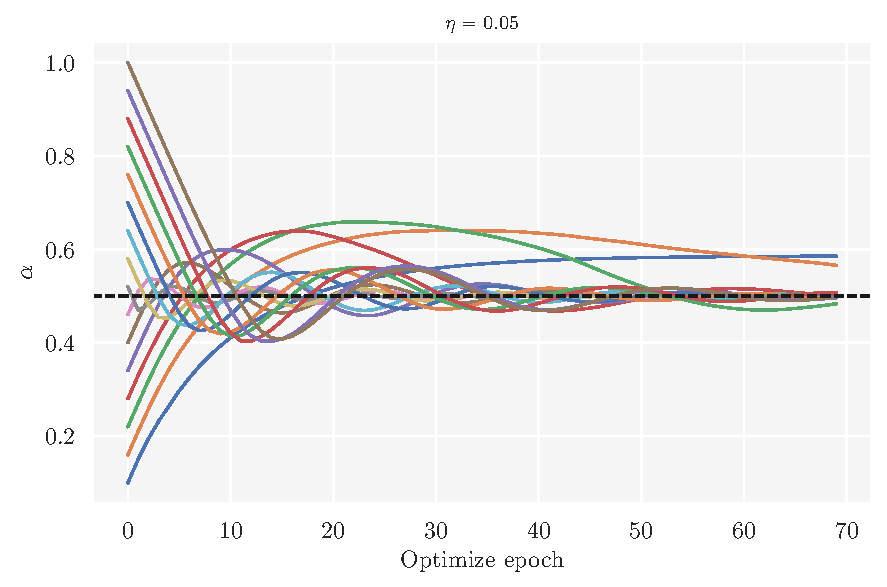
\includegraphics[scale=0.5]{latex/figures/alpha_epoch_lmh_ashonib_eta005.pdf}}}
\qquad
\subfloat[]{{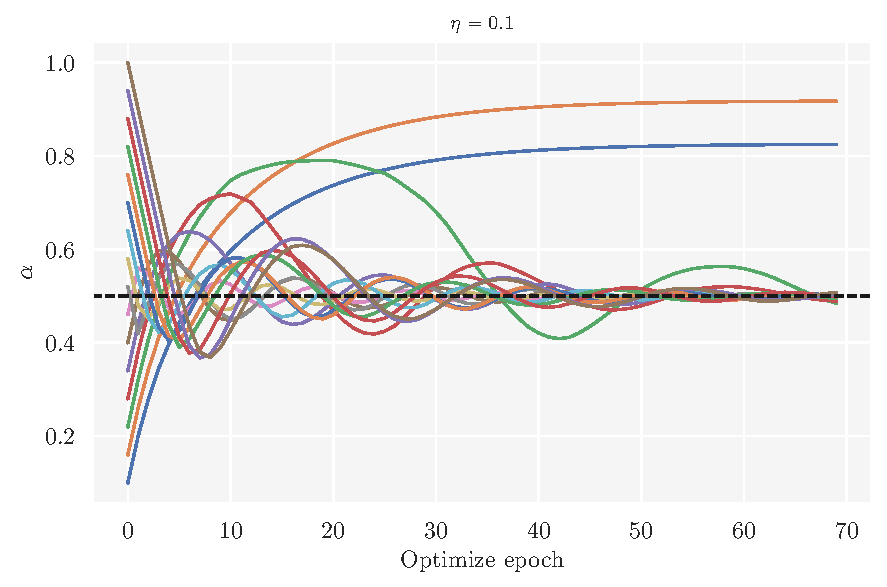
\includegraphics[scale=0.5]{latex/figures/alpha_epoch_lmh_ashonib_eta01.pdf}}}
\qquad
\subfloat[]{{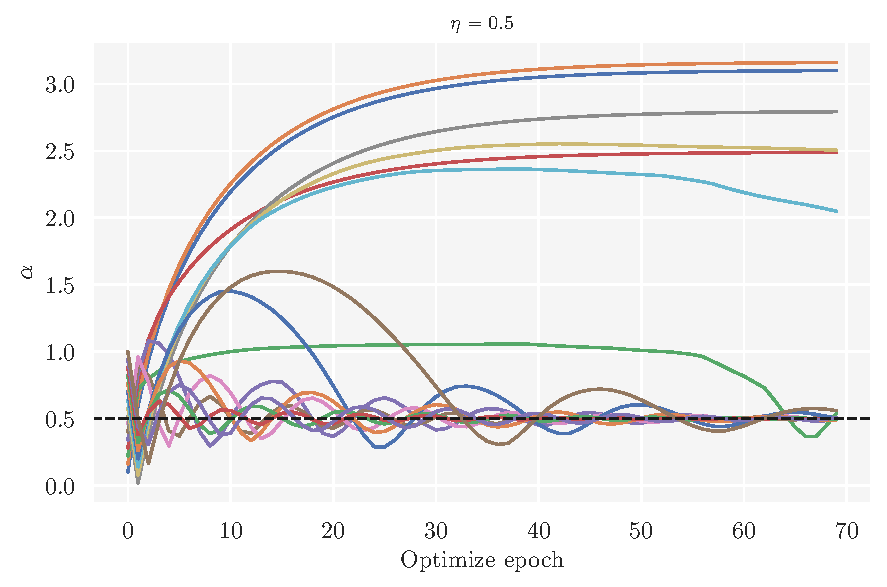
\includegraphics[scale=0.5]{latex/figures/alpha_epoch_lmh_ashonib_eta05.pdf}}}
\caption{figure text}
\label{fig:alpha_epoch_lmh}
\end{figure}

Comparing \autoref{fig:alpha_epoch_rwm} and \autoref{fig:alpha_epoch_lmh} - see no faster convergence of the variational parameter for LMH


\FloatBarrier

%----------------------------------------------------------------
\subsection{Additional Derivations}\label{app:additional_derivations}
%---------------------------------------------------------------

%----------------------------------------------------------------
\subsubsection*{Error in standard Monte Carlo approximation}
%---------------------------------------------------------------- 
The mean square error $\epsilon_M$ of the Monte Carlo approximation can be written as 
\begin{equation}
    \mathcal{E}_M(\mathbb{E}[f(X)],E_M[f]) = \sqrt{\mathbb{E}[(\mathbb{E}[f(X)]-E_M[f])^2]}. 
\end{equation}
First we recognize the fact that the expecation value of the Monte Carlo approximation is equal to the true expectation value,  $\mathbb{E}[f(X_m)]=\mathbb{E}[f(X)]\quad \forall m\in[1, M]\in\mathbb{N}$, which must be true as $X$ and $X_m$ are identically distributed. We denote the true expecation value, $\mathbb{E}[f(X)]=\mu$. 
We square $\mathcal{E}_M$ 
\begin{equation*}
    \begin{split}
        \mathcal{E}_M^2 &= \mathbb{E}[(\mathbb{E}[f(X)]-E_M[f])^2] \\
        &= \mathbb{E}[\mathbb{E}[f(X)]-2\mathbb{E}[f(X)]E_M[f]+E_M[f]^2] \\
        &= \mathbb{E}[f(X)]-2\mathbb{E}[f(X)]\mathbb{E}[E_M[f]]+\mathbb{E}[E_M[f]^2] \\
        &= \mu^2-2\mu\frac{1}{M}\sum_{m=1}^M\mathbb{E}[f(X_m)] + \frac{1}{M^2}\sum_{m=1}^M\sum_{n=1}^M\mathbb{E}[f(X_m)f(X_n)]. \\
    \end{split}
\end{equation*}
We acknowledge the fact that $f(X_m)$ and $f(X_n)$ are indepent variables, and thus
\begin{equation*}
    \begin{split}
        \mathcal{E}_M^2 &= \mu^2-2\mu\frac{1}{M}\sum_{m=1}^M\mathbb{E}[f(X_m)] + \frac{1}{M^2}\sum_{m=1}^M\sum_{n=1}^N\mathbb{E}[f(X_m)]\mathbb{E}[f(X_n)] \\
        &= \mu^2-2\mu\frac{M\mu}{M} + \frac{1}{M^2}\sum_{m=1}^M(\sum_{m\neq n}\mu^2 + \mathbb{E}[f(X)^2]) \\
        &= -\mu^2+\frac{1}{M^2}((M^2-M)\mu^2 + M\mathbb{E}[f(X)^2]) \\
        &= -\frac{\mu^2}{M} + \frac{1}{M}\mathbb{E}[f(X)^2] \\
        &= \frac{\mathbb{E}[f(X)^2]-\mathbb{E}[f(X)]^2}{M} = \frac{\text{Var}[f(X)]}{M} \\
    \end{split}
\end{equation*}
which leads to 
\begin{equation*}
    \mathcal{E}_M = \frac{\sqrt{\text{Var}[f(X)]}}{\sqrt{M}}.
\end{equation*}



%------------------------------------------------------------------
\subsubsection*{Derivation of the gradient of the local energy with respect to the variational parameters.}
%------------------------------------------------------------------

The expected value of the energy is 
\begin{equation}
    \expval{E} = \int\mathrm{d}\bm{r}E_L(\bm{r};\bm{\alpha})p(\bm{r};\bm{\alpha}),
\end{equation}
which can be rewritten as 
\begin{equation}
    \expval{E} = \frac{\int\mathrm{d}\bm{r}\Psi^*H\Psi}{\int\mathrm{d}\bm{r}\Psi^*\Psi}.
\end{equation}
Now we want to take the derivative of this expression with respect to the variational parameters $\bm{\alpha}$. 
\begin{align*}
    \grad_{\bm{\alpha}}\expval{E} &= \frac{\int\mathrm{d}\bm{r}\qty(\grad_{\bm{\alpha}}\Psi^*H\Psi + \Psi^*H\grad_{\bm{\alpha}})}{\int\mathrm{d}\bm{r}\Psi^*\Psi} - \frac{\qty(\int\mathrm{d}\bm{r}\Psi^*H\Psi)\qty(\int\mathrm{d}\bm{r}\qty[\Psi\grad_{\bm{\alpha}}\Psi^* + \Psi^*\grad_{\bm{\alpha}}\Psi])}{\qty(\int\mathrm{d}\bm{r}\Psi^*\Psi)^2} \\
    &(*)= \frac{\int\mathrm{d}\bm{r}\qty(\grad_{\bm{\alpha}}\Psi^*H\Psi + \Psi\qty[H\grad_{\bm{\alpha}}\Psi]^*)}{\int\mathrm{d}\bm{r}\Psi^*\Psi} - 2\expval{E}\expval{\frac{\grad_{\bm{\alpha}}\Psi}{\Psi}} \\
    &= 2\expval{E\frac{\grad_{\bm{\alpha}}\Psi}{\Psi}} - 2\expval{E}\expval{\frac{\grad_{\bm{\alpha}}\Psi}{\Psi}},
\end{align*}
where we assume hermiticity in the Hamiltonian in (*). Thus, the gradient with respect to the variational parameters becomes 
\begin{equation}
    \grad_{\bm{\alpha}}\expval{E} = 2\qty(\expval{E\frac{\grad_{\bm{\alpha}}\Psi}{\Psi}}-\expval{E}\expval{\frac{\grad_{\bm{\alpha}}\Psi}{\Psi}}).
\end{equation}